\section{Prompts}
\label{app:prompts}

\paragraph{Selector.} The \qss{} selector receives the instruction below, followed by the index (or its prefiltered subset) and the question. Its output follows the JSON schema \texttt{\{"rounds": [string]\}}.

\begin{quote}\small
You are the retrieval step of a personal assistant's long-term memory. You get a compact index of the user's entire conversation history (one line per round; images are summarised in a few words) and a question. Choose the rounds that must be opened in full (with their original images) to answer the question. Include EVERY round that may hold needed evidence, especially ALL members of any group the question refers to (e.g. all ads of a brand, every scene of an episode, all versions of a screen over time), not just the best match. Include rounds that define labels the question uses (episode/arc names, `first', `later', `updated'). Image summaries are lossy: when unsure whether an image is relevant, include it. Order by importance. Return JSON with the key ``rounds'' and at most 40 ids.
\end{quote}

\paragraph{Ranking control and LLM rerank.} The ranking control receives the same candidate index lines as the selector and the selector instruction, but ranks all candidates by their need to be opened. The ablation cuts this ranking at eight rounds or at the size that \qss{} chose; the \emph{LLM rerank} baseline gives the reader its top 40 rounds.

\paragraph{Strong widened path.} The strong reader receives the rounds selected by \qss{} and the 40 rounds most similar to the question, in chronological order and without duplicates, together with the cached index on persistent histories.

\paragraph{Per-member notes.} On the widened path, \texttt{gemini-2.5-flash-lite} reads each selected round with its images and extracts facts relevant to the question, including items to total, count, compare, or order, changes of state, and dates for computations. It copies exact numbers, names, labels, and dates and cites each fact's round identifier. The reader receives these notes before the raw rounds.

\paragraph{Reader.} All conditions with the same reader share one system instruction. It asks for concise answers grounded in the provided history and images. The reader should inspect images, use the names given to them in the conversation, prefer the latest evidence when sources conflict, and state when information is absent.

\paragraph{Judges.} On MemEye, the judge uses the official rubric, which scores an answer in $\{0, 0.25, 0.5, 0.75, 1\}$ against the reference answer. On MemLens, the judge uses the official type-specific prompts of the benchmark (binary scores) without modification.

\section{Text Benchmarks and Multimodal Baselines}
\label{app:text}

Figure~\ref{fig:rag_motivation} uses \texttt{gemini-3.8-flash} throughout. LoCoMo uses 100 retrieved turns on 1,540 questions with the earlier answering prompt and lenient binary judge. LongMemEval-S uses 30 rounds on all 500 questions with its official judge; both RAG and full context retain up to 2,000 characters per round. The multimodal RAG runs read the 30 most similar rounds on the question sets of Table~\ref{tab:main}, with the same reader prompt, output cap, and judges as RAG@40. Each RAG/full-context pair uses the same questions and judge. The separate comparisons in Table~\ref{tab:prelim} use the strict judge and settings below.

On LoCoMo and LongMemEval-S, cosine retrieval with a large budget is within one point of full-context reading (Table~\ref{tab:prelim}). On MemEye, top-40 retrieval trails full context by 4.6 points and top-10 retrieval by 14.0, while reading only the annotated evidence trails it by 3.0. Without any visual information, full-context accuracy falls from 0.810 to 0.216.

For the visual-input ablation in Figure~\ref{fig:setsize}b, MemEye and a fixed half of Mem-Gallery use full context with the strong reader; VisualMem uses annotated evidence with the lightweight reader, with chance accuracy of 0.25.

In Table~\ref{tab:prelim}, LoCoMo and LongMemEval-S use the strict LongMemEval judge, while MemEye uses its official 0--1 rubric. The annotated-evidence condition reads only the gold evidence rounds.

\begin{table*}[t]
\centering
\small
\resizebox{\textwidth}{!}{%
\begin{tabular}{llccr}
\toprule
\rowcolor{hHead} Benchmark & Condition & Accuracy & $\Delta$ vs.\ full context & Tokens \\
\midrule
\multirow{3}{*}{LoCoMo (1,540 q)} & Full context & 0.790 & -- & 32,499 \\
 & Cosine top-100 turns & 0.781 & $-0.009$ $[-0.023, +0.006]$ & 5,693 \\
 & Cosine top-10 turns & 0.706 & $-0.084$ $[-0.105, -0.064]$ & 755 \\
\midrule
\multirow{3}{*}{LongMemEval-S (119 q)} & Full context & 0.950 & -- & 113,227 \\
 & Cosine top-50 rounds & 0.941 & $-0.008$ $[-0.034, +0.017]$ & 21,730 \\
 & Cosine top-10 rounds & 0.899 & $-0.050$ $[-0.092, -0.017]$ & 4,986 \\
\midrule
\multirow{5}{*}{MemEye (371 q)} & Full context & 0.810 & -- & 27,220 \\
 & Full context, no visual information & 0.216 & $-0.594$ $[-0.646, -0.542]$ & 11,250 \\
 & Cosine top-40 rounds & 0.764 & $-0.046$ $[-0.075, -0.018]$ & 11,102 \\
 & Cosine top-10 rounds & 0.670 & $-0.140$ $[-0.184, -0.098]$ & 3,914 \\
 & Annotated evidence & 0.780 & $-0.030$ $[-0.069, +0.008]$ & 2,027 \\
\bottomrule
\end{tabular}}
\caption{\textbf{Raw retrieval versus full-context reading.} $\Delta$ is the paired difference from full context with a 95\% bootstrap interval; tokens are prompt tokens per question.}
\label{tab:prelim}
\end{table*}
\section{Robustness}
\label{app:robust}

\paragraph{Pooled estimate.} Over the 837 questions of MemEye and MemLens-32k, the paired gain of \vgs{} over RAG@40 is $+0.046$ $[+0.013, +0.079]$ ($p{=}0.007$) with the lightweight reader and $+0.019$ $[-0.003, +0.040]$ ($p{=}0.09$) with the strong reader.

\paragraph{History-level uncertainty.} Questions that share a history are not independent, so question-level intervals can understate uncertainty. A two-stage bootstrap that resamples histories and then the questions within them gives, for the gain of \vgs{} over RAG@40 with the lightweight and the strong reader, $+0.050$ $[-0.018, +0.120]$ and $+0.029$ $[-0.030, +0.097]$ on the eight MemEye scenarios, $+0.129$ $[+0.066, +0.186]$ and $+0.095$ $[+0.062, +0.134]$ on the ten VisualMem personas, and $+0.103$ $[+0.052, +0.158]$ and $+0.005$ $[-0.019, +0.030]$ on the 20 CamRoll camera rolls. The lightweight-reader gain is positive on 7 of 8, 9 of 10, and 17 of 20 histories. Every MemLens question has its own history.

\paragraph{Selection draws.} The selector thinks at a low level and its sets vary across runs. Three independent selection draws give lightweight-reader accuracies of 0.543, 0.527, and 0.518 on MemEye (standard path) and 0.513, 0.519, and 0.517 on MemLens-32k (widened path); Table~\ref{tab:main} reports the first draw. Averaged over the draws, the gain over RAG@40 is $+0.036$ $[-0.008, +0.080]$ on MemEye, $+0.046$ $[+0.006, +0.087]$ on MemLens, and $+0.042$ $[+0.012, +0.072]$ pooled ($p{=}0.006$).

\paragraph{Reader instruction.} The lightweight reader runs at temperature 0 without thinking, but it is sensitive to its instruction. Removing one example phrase from the reader instruction changed 39\% to 58\% of the MemEye answers and 13\% to 16\% of their scores, in both directions, and moved the accuracy of individual conditions by up to 1.8 points. Differences of this size on MemEye are therefore within the variation between runs.

\paragraph{Second judge.} Qwen3-VL-235B re-scored the MemEye answers with the same rubric. Its scores are lower and preserve the order of the methods: 0.456 for RAG@40, 0.466 for full context, and 0.510 for \vgs{} with the lightweight reader, and 0.710, 0.760, and 0.738 with the strong reader. Exact agreement with the primary judge ranges from 0.77 to 0.84.

\paragraph{Longer MemLens histories.} Table~\ref{tab:memlens_full} repeats the MemLens test split with 64k histories, which have about twice as many rounds. The lightweight-reader gain is 5.8 points ($p{=}0.014$) and the strong-reader gain 1.9 points.

\begin{table}[t]
\centering
\small
\setlength{\tabcolsep}{2.5pt}
\renewcommand{\arraystretch}{1.12}
\begin{tabularx}{\linewidth}{llYYc}
\toprule
\rowcolor{hHead} Reader & History & RAG@40 & \vgs{} & $\Delta$ (points) \\
\midrule
\multirow{2}{*}{Light} & 32k & .470 & \textbf{.513} & $+4.3$ \\
 & 64k & .468 & \textbf{.526} & $+5.8$$^{*}$ \\
\midrule
\multirow{2}{*}{Strong} & 32k & .682 & \textbf{.693} & $+1.1$ \\
 & 64k & .655 & \textbf{.674} & $+1.9$ \\
\bottomrule
\end{tabularx}
\caption{\textbf{MemLens with longer histories (466 test questions).} Accuracy and paired gains over RAG@40 in points; $^{*}$ marks $p<0.05$ in a paired permutation test. Both history lengths use the same questions.}
\label{tab:memlens_full}
\end{table}


\paragraph{Longer histories.} Table~\ref{tab:long} enlarges every MemEye history with image chats of other users, from 126 rounds on average to 1,171 and 4,088, and leaves the questions and their evidence unchanged. \vgs{} still reads the whole index, which grows to 139k tokens. With the strong reader, RAG@40 loses 1.7 to 5.9 points while \vgs{} stays within 2.2 points of its accuracy on the original histories, so its gain grows from 2.9 points to 6.6 and 4.8 ($p{=}0.001$ and $0.02$). With the lightweight reader, \vgs{} remains ahead by 2.6 and 3.0 points, which is not significant. The cost of reading the whole index grows with the history: at 4,088 rounds \vgs{} costs \$12.5 (lightweight) and \$39.2 (strong) per 1,000 questions, against \$0.8 and \$9.6 for RAG@40.

\begin{table}[t]
\centering
\small
\setlength{\tabcolsep}{4pt}
\begin{tabularx}{\linewidth}{lYYYY}
\toprule
\rowcolor{hHead} & \multicolumn{2}{c}{\textbf{Light}} & \multicolumn{2}{c}{\textbf{Strong}} \\
\rowcolor{hHead} \textbf{Rounds} & RAG@40 & \vgs{} & RAG@40 & \vgs{} \\
\midrule
126 & .493 & \textbf{.543} & .764 & \textbf{.793} \\
1,171 & .488 & \textbf{.513} & .705 & \textbf{.771} \\
4,088 & .482 & \textbf{.512} & .747 & \textbf{.795} \\
\bottomrule
\end{tabularx}
\caption{\textbf{Longer histories.} MemEye histories enlarged with image chats of other users (mean rounds per history); the 371 questions and their evidence are unchanged. \vgs{} reads the whole index on its standard path.}
\label{tab:long}
\end{table}


\paragraph{Selector models.} Table~\ref{tab:selectors} compares selector models under the same instruction and compact index. Every selector recovers more complete evidence sets than cosine retrieval with the same number of rounds, by 10 to 34 points. GPT-5-mini comes within one point of the full-set recall of \texttt{gemini-3.8-flash} with 10.1 rounds instead of 7.2, and DeepSeek-V3.1 comes close with 17.6 rounds; lighter models recover fewer sets. End to end with the lightweight reader on MemEye, only \texttt{gemini-3.8-flash} is clearly above RAG@40 (0.543 against 0.493); GPT-5-mini and Qwen3-235B with thinking reach 0.505 and 0.509, and the other selectors fall below RAG@40. On the other benchmarks, GPT-5-mini as the selector gives 0.513 on MemLens-32k (RAG@40: 0.470) and 0.404 on VisualMem (0.450), while DeepSeek-V3.1 and Qwen3-235B do not improve on RAG@40 (0.466 and 0.464 on MemLens; 0.348 and 0.388 on VisualMem). On the 44k-token VisualMem index, these three selectors find the answer-bearing image for 26 to 45\% of the questions, against 80\% for \texttt{gemini-3.8-flash}. The gains of \vgs{} therefore depend on a selector that reads long indexes precisely.

\begin{table}[t]
\centering
\small
\setlength{\tabcolsep}{3.2pt}
\resizebox{\columnwidth}{!}{%
\begin{tabular}{lccc|c}
\toprule
\rowcolor{hHead} \textbf{Selector} & FSR & Rounds & Cosine & Accuracy \\
\midrule
\oursrow gemini-3.8-flash & .860 & 7.2 & .523 & .543 \\
GPT-5-mini & .854 & 10.1 & .615 & .505 \\
DeepSeek-V3.1 & .838 & 17.6 & .739 & .474 \\
gemini-2.5-flash & .712 & 6.2 & .453 & .478 \\
gemini-2.5-flash-lite & .690 & 10.2 & .588 & .480 \\
Qwen3-235B (thinking) & .658 & 5.1 & .445 & .509 \\
Qwen3-235B & .598 & 4.8 & .404 & .477 \\
GPT-4.1-mini & .536 & 4.2 & .391 & .463 \\
\midrule
RAG@40 & .914 & 40 & -- & .493 \\
\bottomrule
\end{tabular}}
\caption{\textbf{Selector models} under the same instruction and compact index on MemEye. FSR and opened rounds of the selection; \emph{Cosine} is the full-set recall of cosine retrieval with as many rounds as each selection; \emph{Accuracy} is the lightweight reader's on the standard path. $^{\ddagger}$A fixed random subset of 150 questions.}
\label{tab:selectors}
\end{table}


\section{Ablation Protocol}
\label{app:dev}

In Table~\ref{tab:ablation}, removing one reading path sends every history to the other; removing the whole index restricts both paths to a 100-round cosine pool. Selection controls use this same pool and the same selector model. The model ranking uses the \qss{} instruction and returns a ranking, cut at either eight rounds or the size chosen by \qss{}; the top-eight control changes both the output rule and the budget. MemLens histories contain at most 83 rounds, so the pool covers the whole history. On CamRoll, which the gate never widens, the pooled row uses the standard path. Full-set recall measures the rounds handed to the reader (Table~\ref{tab:ablation_full}).

\begin{table*}[t]
\centering
\small
\begin{tabularx}{\linewidth}{X|cc|cc|cc|cc}
\toprule
\multirow{2}{*}{\textbf{Reading}} & \multicolumn{2}{c|}{\cellcolor{hME}\textbf{MemEye}} & \multicolumn{2}{c|}{\cellcolor{hML}\textbf{MemLens}} & \multicolumn{2}{c|}{\cellcolor{hVM}\textbf{VisualMem}} & \multicolumn{2}{c}{\cellcolor{hCR}\textbf{CamRoll}} \\
 & \cellcolor{hME}FSR & \cellcolor{hME}Acc. & \cellcolor{hML}FSR & \cellcolor{hML}Acc. & \cellcolor{hVM}FSR & \cellcolor{hVM}Acc. & \cellcolor{hCR}FSR & \cellcolor{hCR}Acc. \\
\midrule
Cosine top-40 (RAG@40) & .914 & .493 & .648 & .470 & .454 & .450 & .865 & .724 \\
Cosine top-$k$, $k$ = size of the \qss{} set & .528 & .465 & .165 & .382 & .259 & .392 & .641 & .753 \\
Model ranking, top 8 & .792 & .500 & .466 & .431 & .553 & .532 & .828 & .799 \\
Model ranking, top $k$, $k$ = size of the \qss{} set & .854 & .504 & .365 & .453 & .546 & .519 & .841 & .829 \\
\midrule
\qss{}, 100-round pool & .876 & .507 & .373 & .453 & .547 & .522 & .845 & .816 \\
\qss{}, whole index (standard path) & .860 & .543 & .373 & .453 & .787 & .569 & .868 & .827 \\
Widened path for every question & .857 & .476 & .270 & .513 & .805 & .579 & .868 & .815 \\
\oursrow \vgs{} (visibility gate) & .860 & .543 & .270 & .513 & .805 & .579 & .868 & .827 \\
\bottomrule
\end{tabularx}
\caption{\textbf{Full ablation with the lightweight reader.} Full-set recall (FSR) of the rounds handed to the reader and answer accuracy. Ranking and matched-size controls use the same 100-round candidate pool as \qss{}; MemLens histories have at most 83 rounds, so the pool is the whole history.}
\label{tab:ablation_full}
\end{table*}


\section{Visibility Analyses}
\label{app:vis}

\paragraph{Gold rounds of MemLens.} MemLens annotates answer sessions and flags the user turns that state the evidence. Evidence images usually appear in another turn of the same session. We count as gold the rounds in an answer session that contain a flagged turn or an evidence image. This gives an average of 5.9 gold rounds per question, including 4.1 with an image.

\paragraph{History visibility.} $H(h)$ averages 0.69 over the eight MemEye histories (0.55 to 0.85), 0.28 over the MemLens histories (0.22 to 0.35 at 32k and 0.24 to 0.31 at 64k), 0.40 over the ten VisualMem personas (0.39 to 0.41), and 0.99 over the 20 CamRoll camera rolls. Figure~\ref{fig:vis}d plots the lightweight-reader gain from widening against $H(h)$.

\paragraph{Routing policies.} Table~\ref{tab:gate} compares the gate with fixed paths and per-question routers. The per-question estimate $\hat v(q)$ takes the ten rounds most similar to the question and averages, over those that share a content word with it, the share of the shared words that the index line shows; it routes a question to the standard path when $\hat v(q)\ge0.7$, which holds for 90\%, 13\%, 27\%, and nearly 100\% of the MemEye, MemLens, VisualMem, and CamRoll questions. The message-length router widens when the user messages in the ten most similar rounds average at least 165 characters; both thresholds were set on the development data. Random routing uses the path shares of $\hat v(q)$. AUC uses $-\hat v(q)$ to rank the questions that gain from widening above those that lose.

\begin{table*}[t]
\centering
\small
\setlength{\tabcolsep}{4pt}
\begin{tabularx}{\linewidth}{X|cccc|cccc}
\toprule
\rowcolor{hHead} & \multicolumn{4}{c|}{\textbf{Lightweight reader}} & \multicolumn{4}{c}{\textbf{Strong reader}} \\
\rowcolor{hHead} \textbf{Policy} & MemEye & MemLens & VisualMem & CamRoll & MemEye & MemLens & VisualMem & CamRoll \\
\midrule
Standard path for every history & 0.543 & 0.453 & 0.569 & 0.827 & 0.793 & 0.584 & 0.925 & 0.899 \\
Widened path for every history & 0.476 & 0.513 & 0.579 & 0.815 & 0.819 & 0.693 & 0.921 & 0.907 \\
\oursrow \vgs{}: history visibility $H(h)\ge0.45$ & 0.543 & 0.513 & 0.579 & 0.827 & 0.793 & 0.693 & 0.921 & 0.899 \\
\midrule
Per-question estimate $\hat v(q)\ge0.7$ & 0.549 & 0.509 & 0.580 & 0.827 & 0.799 & 0.691 & 0.920 & 0.899 \\
Per-question message length & 0.524 & 0.506 & 0.578 & 0.827 & 0.787 & 0.695 & 0.921 & 0.899 \\
Per-question random routing & 0.536 & 0.505 & 0.576 & 0.827 & 0.796 & 0.679 & 0.922 & 0.899 \\
Per-question oracle & 0.628 & 0.579 & 0.638 & 0.861 & 0.856 & 0.742 & 0.944 & 0.927 \\
AUC of $\hat v(q)$ & 0.49 & 0.50 & 0.51 & 0.50 & 0.58 & 0.63 & 0.47 & 0.50 \\
\bottomrule
\end{tabularx}
\caption{\textbf{Routing policies.} Accuracy when every history takes one path, with the history-level gate of \vgs{}, and with per-question routers. Random routing uses the path shares of the per-question estimate; the oracle takes the better path for each question; AUC measures how well $\hat v(q)$ ranks the questions that gain from widening.}
\label{tab:gate}
\end{table*}


\paragraph{Widened paths by reader.} The two readers widen differently because they use added material differently (Table~\ref{tab:swap}). The lightweight reader loses 4.3 and 6.0 points on MemLens and VisualMem when it reads the selected rounds together with the top-40 rounds instead of notes; the strong reader loses 2.6 to 6.5 points on every benchmark when it reads notes instead of the added rounds.

\begin{table}[t]
\centering
\footnotesize
\setlength{\tabcolsep}{2.2pt}
\resizebox{\columnwidth}{!}{%
\begin{tabular}{llccc}
\toprule
\rowcolor{hHead} Reader & Widened path & MemEye & MemLens & VisualMem \\
\midrule
\multirow{2}{*}{Light} & notes + selected rounds & .476 & \textbf{.513} & \textbf{.579} \\
 & selected $\cup$ top-40 rounds & \textbf{.493} & .470 & .519 \\
\midrule
\multirow{2}{*}{Strong} & selected $\cup$ top-40 rounds & \textbf{.819} & \textbf{.693} & \textbf{.921} \\
 & notes + selected rounds & .754 & .667 & .862 \\
\bottomrule
\end{tabular}}
\caption{\textbf{Swapping the widened paths.} Accuracy when each reader uses its own widened path (first row of each block) or the other reader's, applied to every question.}
\label{tab:swap}
\end{table}


\paragraph{Parts of the widened path.} On MemLens-32k with the lightweight reader, longer index lines and notes contribute about equally. The standard path scores 0.453. Lines of 600 characters without notes give 0.483, notes with the standard 200-character lines give 0.489, and both together give 0.513. Lines of 2,000 characters do not help further (0.485).

\paragraph{Shorter index lines.} Truncating the user text on MemEye's index lines to 60 or 30 characters lowers its history visibility from 0.69 to 0.64 and 0.58, which remains above $\tau$. The standard path keeps most of its accuracy (0.526 and 0.529 against 0.543) because image descriptions carry most of the indexed content of these histories.

\section{Retrieval Baselines}
\label{app:retrieval}

Table~\ref{tab:retrieval} varies the retrieval budget and adds two stronger retrievers at the budget of RAG@40. For the strong reader, accuracy rises with the budget on every benchmark. For the lightweight reader, 40 rounds are best on MemEye and VisualMem, 20 on MemLens (0.485), and 10 on CamRoll (0.754); \vgs{} remains 2.8 and 7.3 points above these best budgets. Fusing BM25 with dense retrieval changes accuracy by at most 3 points in either direction; with the strong reader on MemLens it reaches 0.700, above \vgs{} (0.693). Re-ranking the 100 most similar rounds with the selector model raises full-set recall at 40 rounds from 0.91 to 0.98 on MemEye, 0.65 to 0.86 on MemLens, 0.45 to 0.59 on VisualMem, and 0.87 to 0.90 on CamRoll; it helps the strong reader on MemEye and VisualMem and the lightweight reader only on VisualMem. Table~\ref{tab:rerank} sets this baseline beside RAG@40 and \vgs{} on all four benchmarks with its cost: the ranking call makes it more expensive than \vgs{} in seven of the eight settings, and \vgs{} is more accurate in seven, by 0.3 to 9.3 points; with the strong reader on CamRoll the reranker is 0.2 points ahead.

\begin{table*}[t]
\centering
\small
\setlength{\tabcolsep}{2.3pt}
\begin{tabularx}{\linewidth}{l|ccY|ccY|ccY|ccY}
\toprule
\multirow{2}{*}{\textbf{Method}} & \multicolumn{3}{c|}{\cellcolor{hME}\textbf{MemEye}} & \multicolumn{3}{c|}{\cellcolor{hML}\textbf{MemLens}} & \multicolumn{3}{c|}{\cellcolor{hVM}\textbf{VisualMem}} & \multicolumn{3}{c}{\cellcolor{hCR}\textbf{CamRoll}} \\
 & \cellcolor{hME}Light & \cellcolor{hME}Strong & \cellcolor{hME}\$/1k & \cellcolor{hML}Light & \cellcolor{hML}Strong & \cellcolor{hML}\$/1k & \cellcolor{hVM}Light & \cellcolor{hVM}Strong & \cellcolor{hVM}\$/1k & \cellcolor{hCR}Light & \cellcolor{hCR}Strong & \cellcolor{hCR}\$/1k \\
\midrule
RAG@40 & .493 & .764 & 0.9\,/\,9.7 & .470 & .682 & 1.7\,/\,14.0 & .450 & .826 & 1.0\,/\,8.8 & .724 & .894 & 1.3\,/\,11.4 \\
RAG@40 + LLM rerank & .474 & .790 & 6.0\,/\,15.7 & .446 & .674 & 6.4\,/\,22.0 & .499 & .861 & 8.9\,/\,17.7 & .734 & \textbf{.901} & 9.1\,/\,19.2 \\
\oursrow \textbf{\vgs{} (ours)} & \textbf{.543} & \textbf{.793} & 1.6\,/\,5.5 & \textbf{.513} & \textbf{.693} & 4.6\,/\,13.8 & \textbf{.579} & \textbf{.921} & 6.6\,/\,23.1 & \textbf{.827} & .899 & 5.7\,/\,15.7 \\
\bottomrule
\end{tabularx}
\caption{\textbf{Re-ranked retrieval.} Accuracy with the lightweight and the strong reader and cost in USD per 1,000 questions (lightweight\,/\,strong). The selector model re-ranks the 100 most similar rounds and the reader receives the top 40; the cost includes the ranking call.}
\label{tab:rerank}
\end{table*}


\begin{table*}[t]
\centering
\small
\setlength{\tabcolsep}{5pt}
\begin{tabular}{l|cc|cc|cc|cc}
\toprule
\multirow{2}{*}{\textbf{Retrieval}} & \multicolumn{2}{c|}{\cellcolor{hME}\textbf{MemEye}} & \multicolumn{2}{c|}{\cellcolor{hML}\textbf{MemLens}} & \multicolumn{2}{c|}{\cellcolor{hVM}\textbf{VisualMem}} & \multicolumn{2}{c}{\cellcolor{hCR}\textbf{CamRoll}} \\
 & \cellcolor{hME}Light & \cellcolor{hME}Strong & \cellcolor{hML}Light & \cellcolor{hML}Strong & \cellcolor{hVM}Light & \cellcolor{hVM}Strong & \cellcolor{hCR}Light & \cellcolor{hCR}Strong \\
\midrule
Dense top-10 & .449 & .670 & .442 & .543 & .405 & .750 & .754 & .853 \\
Dense top-20 & .475 & .723 & .485 & .624 & .438 & .795 & .749 & .884 \\
Dense top-30 & .479 & .750 & .459 & .652 & .438 & .806 & .730 & .890 \\
Dense top-40 (RAG@40) & .493 & .764 & .470 & .682 & .450 & .826 & .724 & .894 \\
BM25 + dense (RRF), top-40 & .463 & .770 & .459 & .700 & .457 & .836 & .702 & .891 \\
Dense top-100 $\rightarrow$ LLM rerank, top-40 & .474 & .790 & .446 & .674 & .499 & .861 & .734 & .901 \\
\midrule
\oursrow \vgs{} & .543 & .793 & .513 & .693 & .579 & .921 & .827 & .899 \\
\bottomrule
\end{tabular}
\caption{\textbf{Retrieval baselines.} Accuracy with the lightweight and the strong reader. The reranker is the selector model with the selector instruction, applied to the 100 most similar rounds.}
\label{tab:retrieval}
\end{table*}


\section{Cost and Deployment}
\label{app:cost}

\paragraph{Cost model.} Per million tokens, \texttt{gemini-3.8-flash} costs \$0.75 for input, \$0.075 for cached input, and \$3.75 for output including thinking. The corresponding rates for \texttt{gemini-2.5-flash-lite} are \$0.10, \$0.01, and \$0.40. Embeddings cost \$0.20 for text and \$0.45 for images with \texttt{gemini-embedding-2}. We use list prices and the cached-token counts reported by the API. Costs include explicit cache creation and storage, divided over the questions asked of each history. Building the index requires one short caption per image (about \$0.001 with \texttt{gemini-3.8-flash}) and one embedding per round.

\paragraph{Index size.} The index averages 5.8k tokens on a MemEye history, 3.2k on a 32k MemLens history, and 44k on a VisualMem persona or a CamRoll camera roll; the 600-character snippets of the widened path add little on MemEye and VisualMem and raise the MemLens index to 4.0k. On persistent histories, each index is cached once per user and history version.

\paragraph{Index in the reader context.} On persistent histories the strong reader receives the cached index together with the opened rounds. Without it, accuracy falls by 3.5 points on MemEye (0.758 against 0.793 on the standard path) and changes by $+0.9$ points on CamRoll (standard path) and $-0.7$ on VisualMem (widened path), while the cost per question falls by 6\%, 40\%, and 29\%. We keep the index for every history; for photo collections it could be dropped to save cost.

\begin{table}[t]
\centering
\small
\setlength{\tabcolsep}{3pt}
\resizebox{\columnwidth}{!}{%
\begin{tabular}{lcccc}
\toprule
\rowcolor{hHead} \textbf{Method} & MemEye & MemLens & VisualMem & CamRoll \\
\midrule
RAG@40 & 0.9\,/\,9.7 & 1.7\,/\,14.0 & 1.0\,/\,8.8 & 1.3\,/\,11.4 \\
\quad + LLM rerank & 6.0\,/\,15.7 & 6.4\,/\,22.0 & 8.9\,/\,17.7 & 9.1\,/\,19.2 \\
Full context & 0.4\,/\,21.9 & 3.1\,/\,24.9 & 3.2\,/\,154 & --\,/\,-- \\
\midrule
SimpleMem & 12.5\,/\,15.6 & 46.8\,/\,49.0 & 21.8\,/\,26.2 & 23.4\,/\,27.7 \\
Omni-SimpleMem & 2.2\,/\,3.9 & 48.3\,/\,50.4 & 10.5\,/\,13.2 & 15.6\,/\,18.2 \\
TeleMem & 0.7\,/\,2.1 & 30.6\,/\,32.2 & 4.3\,/\,6.3 & 2.0\,/\,4.1 \\
\midrule
V-Mem & 1.0\,/\,9.5 & 1.9\,/\,16.1 & 1.4\,/\,11.0 & 1.3\,/\,11.9 \\
MMA & 2.2\,/\,16.7 & 3.6\,/\,18.8 & 3.0\,/\,22.9 & 5.6\,/\,24.4 \\
\midrule
\oursrow \textbf{\vgs{} (ours)} & 1.6\,/\,5.5 & 4.6\,/\,13.8 & 6.6\,/\,23.1 & 5.7\,/\,15.7 \\
\bottomrule
\end{tabular}}
\caption{\textbf{Cost.} USD per 1,000 questions with the lightweight\,/\,strong reader, including memory construction and caches.}
\label{tab:cost}
\end{table}


\begin{figure*}[t]
\centering
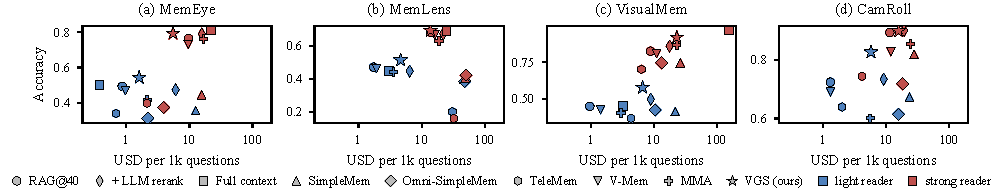
\includegraphics[width=\textwidth]{figures_polished/cost.pdf}
\caption{\textbf{Accuracy and cost.} Total cost per 1,000 questions on the evaluation sets of Table~\ref{tab:main}, including memory construction and caches. Symbols identify methods and colors distinguish readers.}
\label{fig:cost}
\end{figure*}

\section{Reproducibility}
\label{app:repro}

The project repository contains the code, per-question outputs (retrieved rounds, predictions, judge scores and rationales, token usage), and logs. Analysis scripts recompute tables and figures from stored outputs without API calls; new end-to-end runs issue model calls and can produce different outputs. Subsets, samples, and random orders are fixed by stored identifiers and seeds. Prompts and the gate threshold were fixed with MemEye and the 233 MemLens development questions. Two design choices were revised after first runs on MemEye, MemLens, and VisualMem: the gate moved from the question to the history level (Appendix~\ref{app:vis} reports the per-question variant), and the strong reader's widened path adds the 40 most similar rounds. CamRoll was run with the final configuration, and all reported results use this single configuration.

\section{VisualMem and CamRoll Details}
\label{app:visualmem}

\paragraph{Data.} VisualMem~\citep{nguyen2026personalvisual} has ten personas, each with about 171 dated events containing one shared image. Its 696 multiple-choice questions each have four options; 631 use text options and 65 use image options, and six include a query image. Questions concern facts placed only in earlier images or recurring entities. We treat each event as a session and each user turn plus the following assistant turn as a round. All questions are asked after the full history. The gold rounds are the image rounds of the event associated with the question. For every method, we downscale images to 1,024 pixels on the longer side and score the first option letter against the gold letter.

\paragraph{Visual dependence.} Removing all visual information (images and their descriptions) shows how much the questions depend on images. With the annotated evidence, accuracy falls from 0.609 to 0.297, close to the chance level of 0.25. Top-40 retrieval keeps 91\% of its accuracy without visual information; it retrieves the evidence round for 45.4\% of the questions.

\paragraph{CamRoll.} CamRoll-yfcc20~\citep{nguyen2026camroll} provides 20 personal camera rolls sampled from YFCC100M, with 505 to 979 photos per roll (780 on average, 15,607 in total) taken on 225 different days on average. Each roll has 10 questions about the album owner and 40 about specific photos, with three options each; the released files list the correct option first, so we shuffle the options with a seed derived from the question identifier. Gold rounds are the photos that an episodic question references. We treat each photo as a round whose text is its capture time, group the photos of a calendar day into a session, and give every reader the owner's reference photo. Because an index line shows the capture time and the photo's description in full, history visibility is 0.99 for every roll and the gate selects the standard path. Embedding similarity ranks 74\% of the gold photos among the ten most similar rounds and 11\% beyond the top 40. Full-context reading would send about 800 photos (245k tokens for the lightweight reader) with every question and was not run.

\section{Standard Metrics and Latency}
\label{app:latency}

\begin{table*}[t]
\centering
\footnotesize
\setlength{\tabcolsep}{2.4pt}
\begin{tabular}[t]{l|cc|cc}
\toprule
\rowcolor{hHead} & \multicolumn{2}{c|}{\textbf{Token F1}} & \multicolumn{2}{c}{\textbf{BLEU-1}} \\
\rowcolor{hHead} \textbf{Method} & MemEye & MemLens & MemEye & MemLens \\
\midrule
RAG@40 & .299 / .505 & .414 / .560 & .251 / .441 & .397 / .534 \\
SimpleMem & .236 / .297 & .335 / .338 & .194 / .258 & .321 / .325 \\
Omni-SimpleMem & .218 / .272 & .331 / .342 & .180 / .239 & .317 / .327 \\
TeleMem & .248 / .279 & .207 / .131 & .210 / .243 & .197 / .125 \\
V-Mem & .303 / .482 & .402 / .546 & .259 / .418 & .385 / .515 \\
MMA & .286 / .499 & .389 / .534 & .238 / .440 & .370 / .505 \\
\midrule
\oursrow \vgs{} (ours) & \textbf{.351} / \textbf{.514} & \textbf{.436} / \textbf{.578} & \textbf{.303} / \textbf{.449} & \textbf{.415} / \textbf{.552} \\
\bottomrule
\end{tabular}\hfill
\begin{tabular}[t]{l|ccc|ccc}
\toprule
\rowcolor{hHead} & \multicolumn{3}{c|}{\textbf{Recall@10}} & \multicolumn{3}{c}{\textbf{nDCG@10}} \\
\rowcolor{hHead} \textbf{Method} & ME & ML & VM & ME & ML & VM \\
\midrule
RAG@40 & .790 & .584 & .297 & .676 & .548 & .225 \\
V-Mem & .572 & .594 & .256 & .361 & .455 & .195 \\
MMA & .697 & \textbf{.800} & .355 & .550 & \textbf{.808} & .246 \\
\midrule
\oursrow \vgs{} (ours) & \textbf{.879} & .620 & \textbf{.793} & \textbf{.803} & .714 & \textbf{.699} \\
\bottomrule
\end{tabular}
\caption{\textbf{Standard metrics on MemEye, MemLens, and VisualMem.} Left, answer metrics for lightweight / strong readers. Right, evidence metrics for methods returning raw rounds, using the lightweight path for \vgs{}. Definitions are in Appendix~\ref{app:latency}.}
\label{tab:std}
\end{table*}


\paragraph{Answer metrics.} We compute token F1 and BLEU-1 following the LoCoMo evaluation (Table~\ref{tab:std}). We lowercase answers and references, remove punctuation and articles, and split tokens on white space. BLEU-1 uses clipped unigram precision with the brevity penalty.

\paragraph{Evidence metrics.} Recall@10 is the fraction of all gold evidence rounds recovered within the first ten retrieved rounds. We use cosine rank for top-40 retrieval, the selector's order for \vgs{}, and the returned order for V-Mem and MMA. nDCG@10 uses binary relevance.

\paragraph{Latency.} We time each question from receipt to the reader's answer, with the memory already built. Questions run one at a time on the same machine and network. The samples contain 30 questions from one MemEye history (120 rounds), 10 MemLens-32k questions with separate histories, and 30 questions from one VisualMem persona (1,013 rounds). Each method runs its own retrieval, including model calls, followed by the common reader call. We exclude the first question of a persistent history because it creates the context cache. About 3\% of each method's calls stalled until the 240-s client timeout and were retried, so we report medians (Table~\ref{tab:latency}). Construction times use each system's default parallelism; MemLens construction time is the median over the ten histories.

\begin{table*}[t]
\centering
\small
\setlength{\tabcolsep}{3.2pt}
\resizebox{\textwidth}{!}{%
\begin{tabular}{l|cc|cc|cc|ccc}
\toprule
\rowcolor{hHead} & \multicolumn{2}{c|}{\cellcolor{hME}\textbf{MemEye}} & \multicolumn{2}{c|}{\cellcolor{hML}\textbf{MemLens}} & \multicolumn{2}{c|}{\cellcolor{hVM}\textbf{VisualMem}} & \multicolumn{3}{c}{\textbf{Construction (s per history)}} \\
\rowcolor{hHead} \textbf{Method} & Answer & Retrieval & Answer & Retrieval & Answer & Retrieval & MemEye & MemLens & VisualMem \\
\midrule
RAG@40 & 5.4 / 8.8 & 1.2 & 16.5 / 9.9 & 1.7 & 15.7 / 8.4 & 1.6 & 20.4 & 10.9 & 44.7 \\
SimpleMem & 22.0 / 22.5 & 20.5 & 22.6 / 23.1 & 21.3 & 23.8 / 25.2 & 21.8 & 158 & 38.8 & 808 \\
Omni-SimpleMem & 3.0 / 4.2 & 1.7 & 4.2 / 4.0 & 1.4 & 5.5 / 8.0 & 3.6 & 685 & 172 & 2,701 \\
V-Mem & 3.2 / 6.1 & 0.0 & 2.1 / 8.4 & 0.0 & 1.9 / 5.7 & 0.0 & 0.4 & 0.6 & 5.8 \\
MMA & 5.5 / 10.4 & 0.0 & 2.3 / 4.5 & 0.0 & 5.4 / 10.2 & 0.0 & 632 & 21.1 & 276 \\
TeleMem & 2.0 / 3.3 & 0.9 & 3.9 / 3.8 & 1.2 & 1.8 / 3.0 & 0.8 & 86.3 & 38.2 & 507 \\
\midrule
\oursrow \vgs{} (ours) & 5.0 / 8.9 & 3.6 & 8.8 / 8.6 & 4.3 & 11.0 / 14.0 & 5.9 & 20.4 & 10.9 & 44.7 \\
\bottomrule
\end{tabular}}
\caption{\textbf{Latency and construction time in seconds.} Answer latency uses the lightweight / strong reader. Retrieval includes model calls, and construction is per history. Sample sizes and timing protocols are in Appendix~\ref{app:latency}.}
\label{tab:latency}
\end{table*}


\section{External Memory Systems}
\label{app:baselines}

The five systems use released code with the retrieval budgets and adaptations in Table~\ref{tab:systems}. MMA uses the implementation in the official MemEye evaluation framework. Each system builds one memory per history from the same dated rounds, in chronological order, and the same image descriptions. Multimodal systems also receive the raw images. Construction uses \texttt{gemini-3.8-flash} with low thinking, except for the roles listed in the table, and image embeddings use \texttt{gemini-embedding-2}. Each system retrieves from the full question text using its own method. Retrieved records and any returned images go to the same reader prompt, answer format, and judges. Costs include construction, divided over each benchmark's questions.

\begin{table*}[t]
\centering
\small
\setlength{\tabcolsep}{3.4pt}
\begin{tabularx}{\linewidth}{>{\raggedright\arraybackslash}p{2.6cm}|>{\raggedright\arraybackslash}p{3.8cm}|>{\raggedright\arraybackslash}p{3.0cm}|>{\raggedright\arraybackslash}p{2.5cm}|>{\raggedright\arraybackslash}X}
\toprule
\rowcolor{hHead} \textbf{System} & \textbf{Memory written at ingestion} & \textbf{Retrieval (budget)} & \textbf{Other models} & \textbf{Adaptation} \\
\midrule
SimpleMem (0.3.0) & factual statements from windows of 40 turns, with resolved references and times & planning, reflection, hybrid search & -- & punctuation removed from keyword queries \\
Omni-SimpleMem (0.3.0) & multimodal atomic units, knowledge graph; images as on-demand units & hybrid search, graph expansion (20 units) & unit summaries (2.5-flash-lite) & no modality filter for questions about images \\
TeleMem (1.10.1) & one memory per message, for the user profile and for events & top 30 per scope & extraction (2.5-flash-lite) & English extraction prompts \\
V-Mem & raw user, assistant, and image units of every round & modality routing (20 rounds and neighbours) & anchors (2.5-flash-lite) & -- \\
MMA & raw turns with a confidence score & similarity $\times$ confidence (80 turns) & -- & -- \\
\bottomrule
\end{tabularx}
\caption{\textbf{External memory systems.} ``Other models'' lists roles that do not use \texttt{gemini-3.8-flash}; ``Adaptation'' lists the changes needed to run each release on our data.}
\label{tab:systems}
\end{table*}


\begin{figure*}[t]
\centering
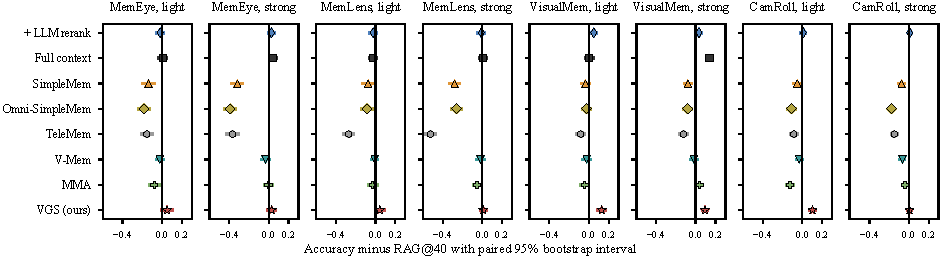
\includegraphics[width=\textwidth]{figures_polished/app_baselines.pdf}
\caption{Paired difference of every method from RAG@40 with 95\% bootstrap intervals on the question sets of Table~\ref{tab:main}.}
\label{fig:app_baselines}
\end{figure*}
